\chapter{Deadlock}

\epigraph{No, you can't always get what you want
	\\You can't always get what you want
	\\You can't always get what you want
	\\But if you try sometimes you find
	\\You get what you need}{The philosophers Jagger \& Richards}

\gls{Deadlock} is defined as when a system cannot make and forward progress.
We define a system for the rest of the chapter as a set of rules by which a set of processes can move from one state to another, where a state is either working or waiting for a particular resource.
Forward progress is defined as if there is at least one process working or we can award a process waiting for a resource that resource.
In a lot of systems, Deadlock is avoided by ignoring the entire concept \cite[P.237]{silberschatz2006operating}.
Have you heard about turn it on and off again?
For products where the stakes are low (User Operating Systems, Phones), it may be more efficient to allow deadlock.
But in the cases where ``failure is not an option'' - Apollo 13, you need a system that tracks, breaks, or prevents deadlocks.
Apollo 13 didn't fail because of deadlock, but it wouldn't be good to restart the system on liftoff.

Mission-critical operating systems need this guarantee formally because playing the odds with people's lives isn't a good idea.
Okay so how do we do this? We model the problem.
Even though it is a common statistical phrase that all models are wrong, the more accurate the model is to the system the higher the chance the method will work.

\section{Resource Allocation Graphs}

\begin{figure}[H]
	\centering
	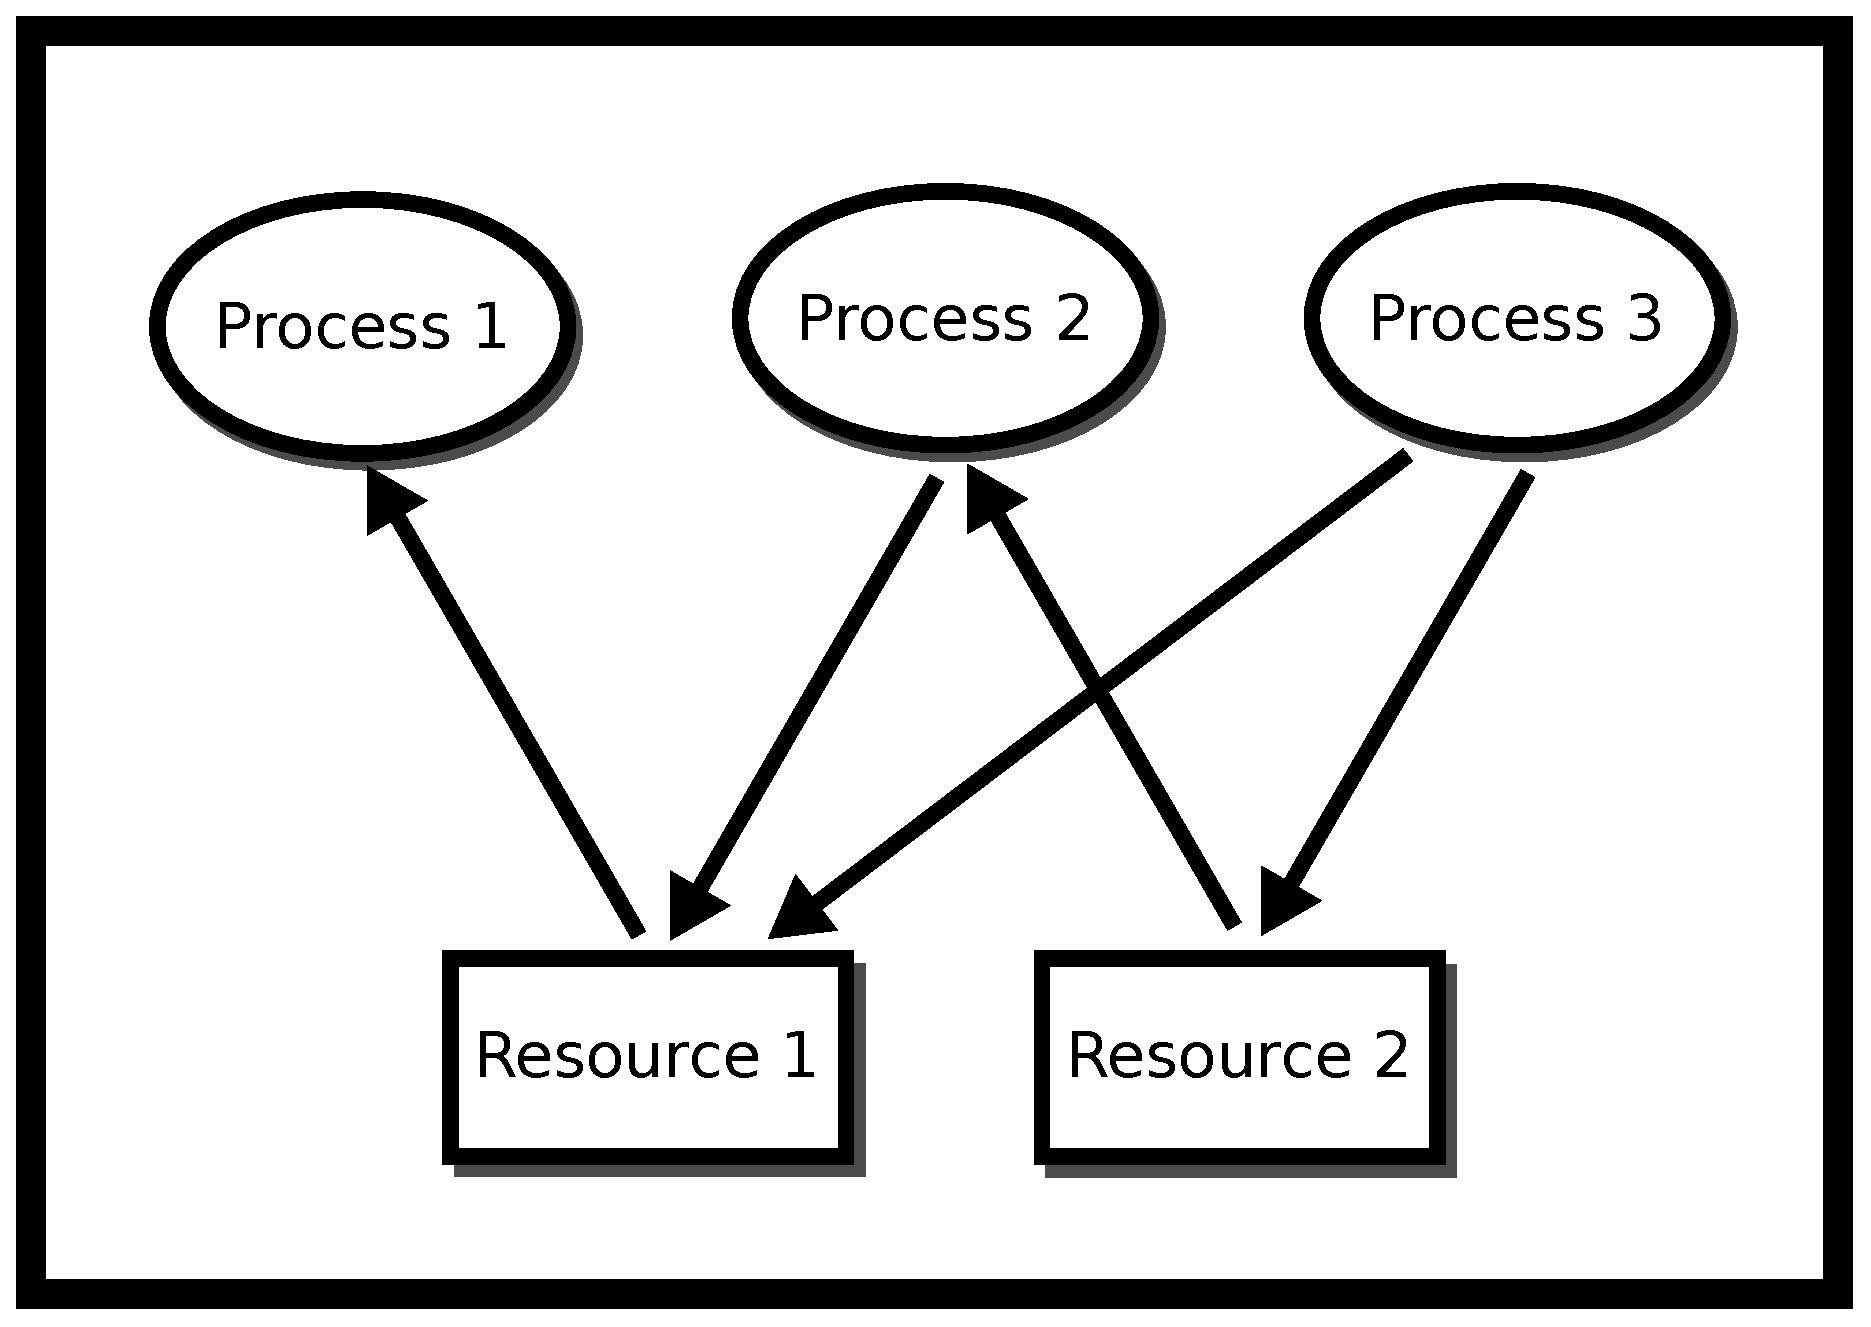
\includegraphics[width=.6\textwidth]{deadlock/drawings/rag.eps}
	\caption{Resource allocation graph}
	\label{ragfigure}
\end{figure}

One such way is modeling the system with a resource allocation graph (\gls{RAG}).
A resource allocation graph tracks which resource is held by which process and which process is waiting for a resource of a particular type.
It is a simple yet powerful tool to illustrate how interacting processes can deadlock.
If a process is \emph{using} a resource, an arrow is drawn from the resource node to the process node.
If a process is \emph{requesting} a resource, an arrow is drawn from the process node to the resource node.
If there is a cycle in the Resource Allocation Graph and each resource in the cycle provides only one instance, then the processes will deadlock.
For example, if process 1 holds resource A, process 2 holds resource B and process 1 is waiting for B and process 2 is waiting for A, then processes 1 and 2 will be deadlocked \ref{ragfigure}.
We'll make the distinction that the system is in deadlock by definition if all workers cannot perform an operation other than waiting.
We can detect a deadlock by traversing the graph and searching for a cycle using a graph traversal algorithm, such as the Depth First Search (DFS).
This graph is considered as a directed graph and we can treat both the processes and resources as nodes.

\begin{minted}{C}
	typedef struct {
		int node_id; // Node in this particular graph
		Graph **reachable_nodes; // List of nodes that can be reached from this node
		int size_reachable_nodes; // Size of the List
	} Graph;
	
	// isCyclic() traverses a graph using DFS and detects whether it has a cycle
	// isCyclic() uses a recursive approach
	// G points to a node in a graph, which can be either a resource or a process
	// is_visited is an array indexed with node_id and initialized with zeros (false) to record whether a particular node has been visited
	int isCyclic(Graph *G, int* is_visited) {
		if (this graph has been visited) {
			// Oh! the cycle is found
			return true;
			} else {
			1. Mark this node as visited
			2. Traverse through all nodes in the reachable_nodes
			3. Call isCyclic() for each node
			4. Evaluate the return value of isCyclic()
		}
		// Nope, this graph is acyclic
		return false;
	}
\end{minted}

\begin{figure}[H]
	\centering
	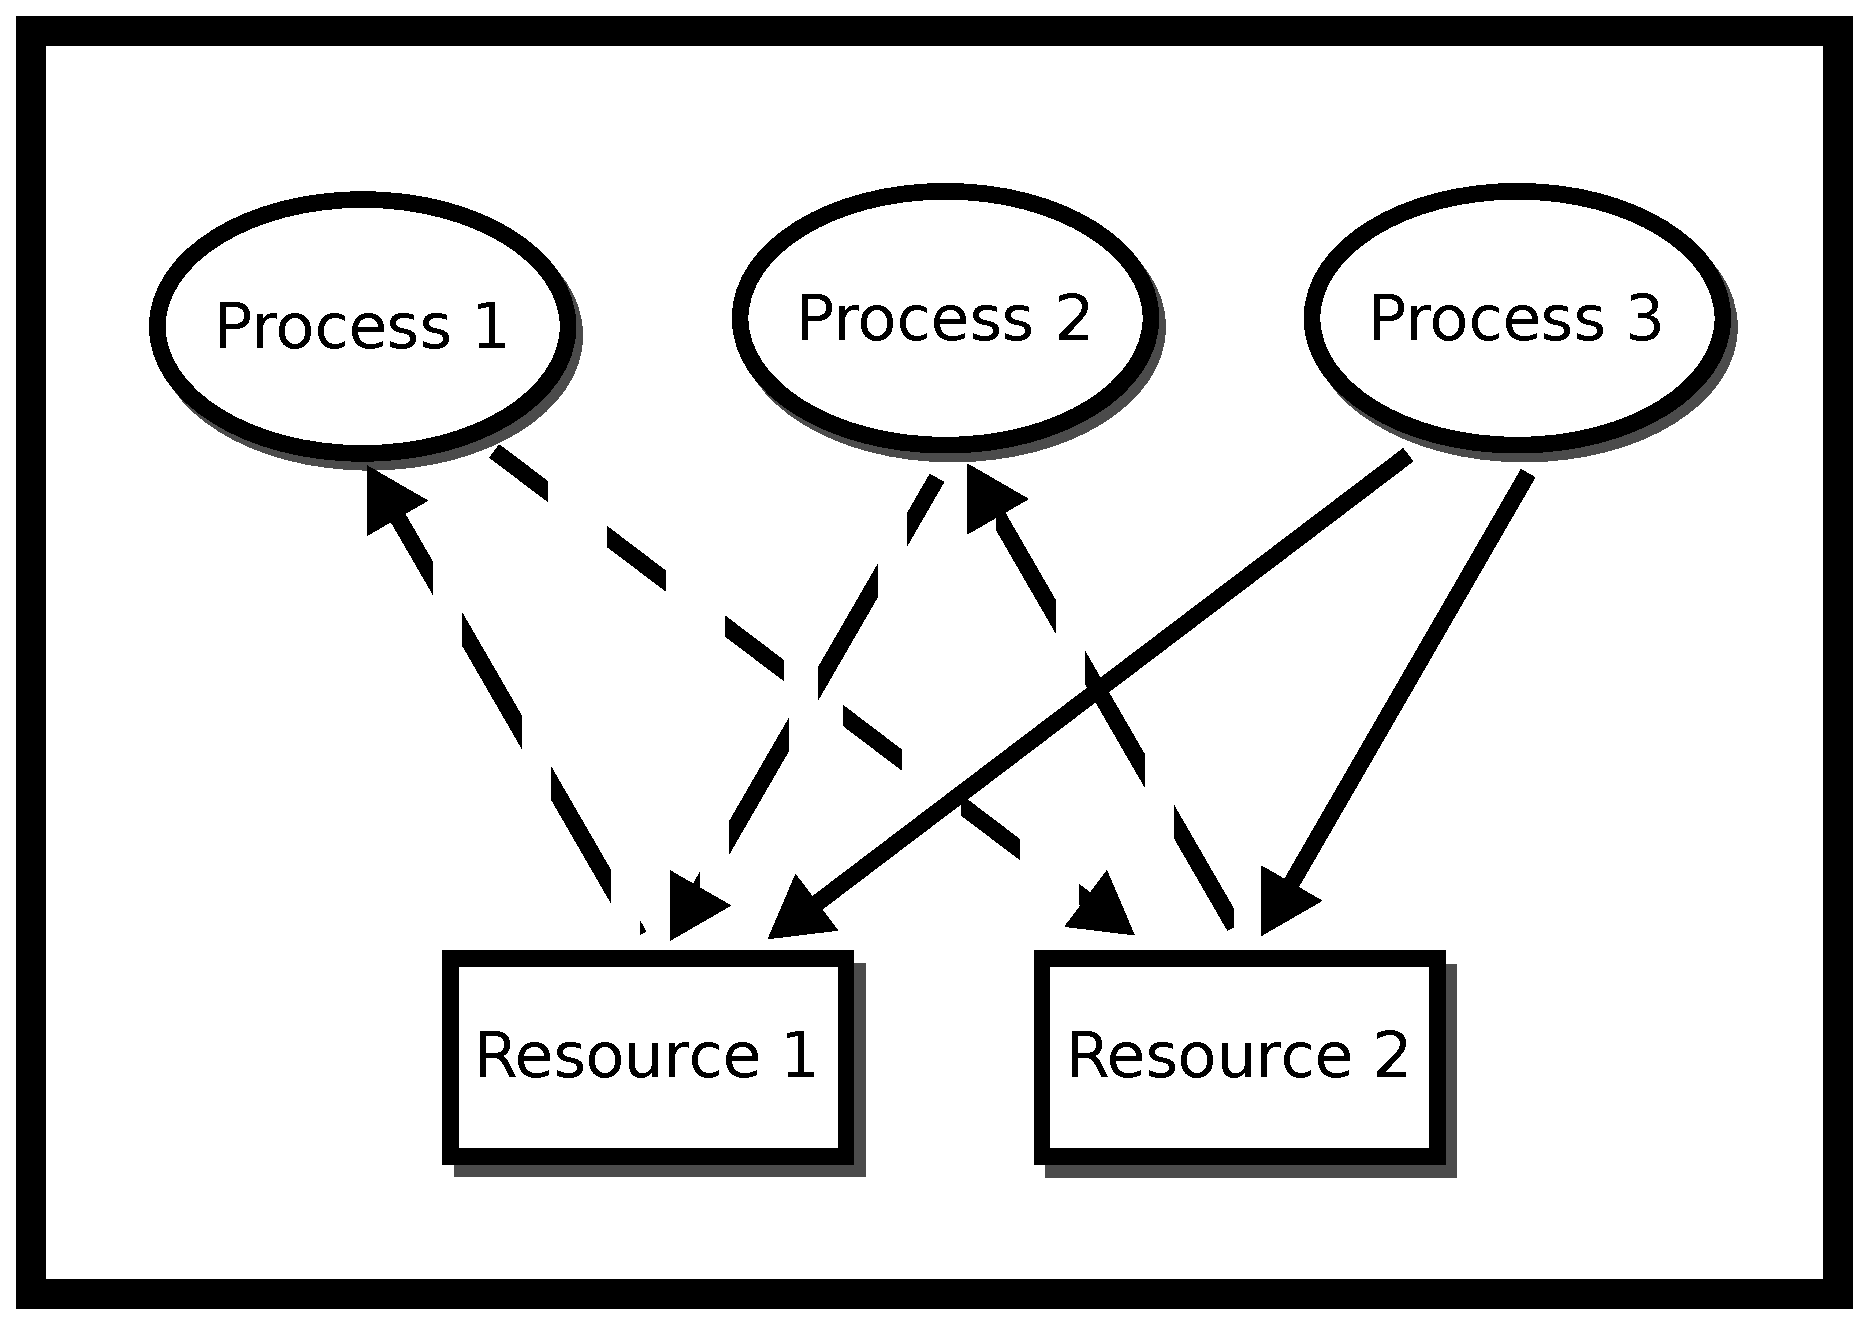
\includegraphics[width=.5\textwidth]{deadlock/drawings/deadlock.eps}
	\caption{Graph based Deadlock}
\end{figure}

\section{Coffman Conditions}

Surely cycles in RAGs happen all the time in an OS, so why doesn't it grind to a halt?
You may not see deadlock because the OS may \textbf{preempt} some processes breaking the cycle but there is still a chance that your three lonely processes could deadlock.

There are four \emph{necessary} and \emph{sufficient} conditions for deadlock -- meaning if these conditions hold then there is a non-zero probability that the system will deadlock at any given iteration.
These are known as the \gls{Coffman Conditions} \cite{coffman1971system}.

\begin{itemize}
	\tightlist
	\item
	      \gls{Mutual Exclusion}: No two processes can obtain a resource at the same time.
	\item
	      \gls{Circular Wait}: There exists a cycle in the Resource Allocation Graph, or there exists a set of processes \{P1, P2,\ldots{}\} such that P1 is waiting for resources held by P2, which is waiting for P3,\ldots{}, which is waiting for P1.
	\item
	      \gls{Hold and Wait}: Once a resource is obtained, a process keeps the resource locked.
	\item
	      No \gls{pre-emption}: Nothing can force the process to give up a resource.
\end{itemize}

\begin{proof} Deadlock can happen if and only if the four Coffman conditions are satisfied.
	
	$\rightarrow$ If the system is deadlocked, the four Coffman conditions are apparent.
	
	\begin{itemize}
		\item For contradiction, assume that there is no circular wait. If not then that means the resource allocation graph is acyclic, meaning that there is at least one process that is not waiting on any resource to be freed. Since the system can move forward, the system is not deadlocked.
		\item For contradiction, assume that there is no mutual exclusion. If not, that means that no process is waiting on any other process for a resource. This breaks circular wait and the previous argument proves correctness.
		\item For contradiction, assume that processes don't hold and wait but our system still deadlocks. Since we have circular wait from the first condition at least one process must be waiting on another process. If that and processes don't hold and wait, that means one process must let go of a resource. Since the system has moved forward, it cannot be deadlocked.
		\item For contradiction, assume that we have preemption, but the system cannot be un-deadlocked. Have one process, or create one process, that recognizes the circular wait that must be apparent from above and break one of the links. By the first branch, we must not have deadlocked.
	\end{itemize}
	
	$\leftarrow$ If the four conditions are apparent, the system is deadlocked.
	We will prove that if the system is not deadlocked, the four conditions are not apparent.
	Though this proof is not formal, let us build a system with the three requirements not including circular wait.
	Let assume that there is a set of processes $P = \{p_1, p_2, ..., p_n\}$ and there is a set of resources $R = \{r_1, r_2, ..., r_m\}$.
	For simplicity, a process can only request one resource at a time but the proof can be generalized to multiple.
	Let assume that the system is a state at time $t$.
	Let us assume that the state of the system is a tuple $(h_t, w_t)$ where there are two functions $h_t: R \rightarrow P \cup \{\text{unassigned}\}$ that maps resources to the processes that own them (this is a function, meaning that we have mutual exclusion) and or unassigned and $w_t: P \rightarrow R \cup \{\text{satisfied}\}$ that maps the requests that each process makes to a resource or if the process is satisfied.
	If the process is satisfied, we consider the work trivial and the process exits, releasing all resources -- this can also be generalized.
	Let $L_t \subseteq P \times R$ be a set of lists of requests that a process uses to release a resource at any given time.
	The evolution of the system is at each step at every time.
	
	\begin{itemize}
		\item Release all resources in $L_t$.
		\item Find a process that is requesting a resource
		\item If that resource is available give it to that process, generating a new $(h_{t+1}, w_{t+1})$ and exit the current iteration.
		\item Else find another process and try the same resource allocation procedure in the previous step.
	\end{itemize}
	
	If all processes have been surveyed and if all are requesting a resource and none can be granted a resource, consider it deadlocked.
	More formally, this system is deadlocked means if $\exists t_0, \forall t \geq t_0, \forall p \in P, w_t(p) \neq \text{satisfied} \text{ and } \exists q, q \neq p \rightarrow h_t(w_t(p)) = q$ (which is what we need to prove).
	
	Mutual exclusion and no pre-emption are encoded into the system.
	Circular wait implies the second condition, a resource is owned by another process which is owned by another process meaning at this state $\forall p \in P, \exists q \neq p \rightarrow h_t(w_t(p)) = q$.
	Circular wait also implies that at this current state, no process is satisfied, meaning at this state $\forall p \in P, w_t(p) \neq \text{satisfied}$.
	Hold and wait simply proves the condition that from this point onward, the system will not change, which is all the conditions that we needed to show.
\end{proof}

If a system breaks any of them, it cannot have deadlock!
Consider the scenario where two students need to write both pen and paper and there is only one of each.
Breaking mutual exclusion means that the students share the pen and paper.
Breaking circular wait could be that the students agree to grab the pen then the paper.
As proof by contradiction, say that deadlock occurs under the rule and the conditions.
Without loss of generality, that means a student would have to be waiting on a pen while holding the paper and the other waiting on a pen and holding the paper.
We have contradicted ourselves because one student grabbed the paper without grabbing the pen, so deadlock fails to occur.
Breaking hold and wait could be that the students try to get the pen and then the paper and if a student fails to grab the paper then they release the pen.
This introduces a new problem called \textit{livelock} which will be discussed later.
Breaking preemption means that if the two students are in deadlock the teacher can come in and break up the deadlock by giving one of the students a held item or tell both students to put the items down.

\gls{livelock} relates to deadlock.
Consider the breaking hold-and-wait solution as above.
Though deadlock is avoided, if the philosopher picks up the same device again and again in the same pattern, no work will be done.
Livelock is generally harder to detect because the processes generally look like they are working to the outside operating system whereas in deadlock the operating system generally knows when two processes are waiting on a system-wide resource.
Another problem is that there are necessary conditions for livelock (i.e. deadlock fails to occur) but not sufficient conditions -- meaning there is no set of rules where livelock has to occur.
You must formally prove in a system by what is known as an invariant.
One has to enumerate each of the steps of a system and if each of the steps eventually -- after some finite number of steps -- leads to forward progress, the system fails to livelock.
There are even better systems that prove bounded waits; a system can only be livelocked for at most $n$ cycles which may be important for something like stock exchanges.

\section{Approaches to Solving Livelock and Deadlock}

Ignoring deadlock is the most obvious approach.
Quite humorously, the name for this approach is called the \gls{ostrich algorithm}.
Though there is no apparent source, the idea for the algorithm comes from the concept of an ostrich sticking its head in the sand.
When the operating system detects deadlock, it does nothing out of the ordinary, and any deadlock usually goes away.
An operating system preempts processes when stopping them for context switches.
The operating system can interrupt any system call, potentially breaking a deadlock scenario.
The OS also makes some files read-only thus making the resource shareable.
What the algorithm refers to is that if there is an adversary that specifically crafts a program -- or equivalently a user who poorly writes a program -- that the OS deadlocks.
For everyday life, this tends to be fine.
When it is not we can turn to the following method.

Deadlock detection allows the system to enter a deadlocked state.
After entering, the system uses the information to break deadlock.
As an example, consider multiple processes accessing files.
The operating system can keep track of all of the files/resources through file descriptors at some level either abstracted through an API or directly.
If the operating system detects a directed cycle in the operating system file descriptor table it may break one process' hold through scheduling for example and let the system proceed.
Why this is a popular choice in this realm is that there is no way of knowing which resources a program will select without running the program.
This is an extension of Rice's theorem \cite{rice} that says that we cannot know any semantic feature without running the program (semantic meaning like what files it tries to open).
So theoretically, it is sound.
The problem then gets introduced that we could reach a livelock scenario if we preempt a set of resources again and again.
The way around this is mostly probabilistic.
The operating system chooses a random resource to break \keyword{hold-and-wait}.
Now even though a user can craft a program where breaking hold and wait on each resource will result in a livelock, this doesn't happen as often on machines that run programs in practice or the livelock that does happen happens for a couple of cycles.
These systems are good for products that need to maintain a non-deadlocked state but can tolerate a small chance of livelock for a short time.

\subsection{Extra: Banker's Algorithm}

We can start with a single resource Banker's Algorithm.
Consider a banker, who has a finite amount of money.
With a finite amount of money, she wants to make loans and eventually get her money back.
Let's say that we have a set of $n$ people where each of them has a set amount or a limit $a_i$ ($i$ being the $i$th process) that they need to obtain before they can do any work.
The banker keeps track of how much she has given to each person $l_i$. She maintains an amount of money $p$ with her, at all times.
For people to request money, they do the following:
Consider the state of the system $(A=\{a_1, a_2, ...\}, L_t=\{l_{t,1}, l_{t,2}, ...\}, p)$ at time $t$.
A precondition is that we have $p \geq min(A)$, or we have enough money to suit at least one person.
Also, each person will work for a finite period and give back our money.

\begin{itemize}
	\item A person $j$ requests $m$ from me
	      \begin{itemize}
	      	\item if $m \geq p$, they are denied.
	      	\item if $m + l_j > a_i$ they are denied
	      	\item Pretend we are in a new state $(A, L_{t+1}=\{.., l_{t+1, j} = l_{t, j} + m, ...\}, p - m)$ where the process is granted the resource.
	      \end{itemize}
	\item if now person $j$ is either satisfied ($l_{t+1,j} == a_j$) or $min(a_i - l_{t+1, i}) \leq p$. In other words, we have enough money to suit one other person. If either, consider the transaction safe and give them the money.
\end{itemize}

Why does this work? Well at the start we are in a safe state -- defined by we have enough money to suit at least one person.
Each of these "loans" results in a safe state.
If we have exhausted our reserve, one person is working and will give us money greater than or equal to our previous "loan", thus putting us in a safe state again.
Since we can always make one additional move, the system can never deadlock.
Now, there is no guarantee that the system won't livelock.
If the process we hope to request something never does, no work will be done -- but not due to deadlock.
This analogy expands to higher orders of magnitude but requires that either a process can do its work entirely or there exists a process whose combination of resources can be satisfied, which makes the algorithm a little more tricky (an additional for loop) but nothing too bad.
There are some notable downsides.

\begin{itemize}
	\item The program first needs to know how much of each resource a process needs. A lot of times that is impossible or the process requests the wrong amount because the programmer didn't foresee it.
	\item The system could livelock.
	\item We know in most systems that resources vary, pipes and sockets for example. This could mean that the runtime of the algorithm could be slow for systems with millions of resources.
	\item Also, this can't keep track of the resources that come and go. A process may delete a resource as a side effect or create a resource. The algorithm assumes a static allocation and that each process performs a non-destructive operation.
\end{itemize}

\section{Dining Philosophers}

The Dining Philosophers problem is a classic synchronization problem.
Imagine we invite $n$ (let's say 6) philosophers to a meal.
We will sit them at a table with 6 chopsticks, one between each philosopher.
A philosopher alternates between wanting to eat or think.
To eat the philosopher must pick up the two chopsticks either side of their position.
The original problem required each philosopher to have two forks, but one can eat with a single fork so we rule this out.
However, these chopsticks are shared with his neighbor.

\begin{figure}[H]
	\centering
	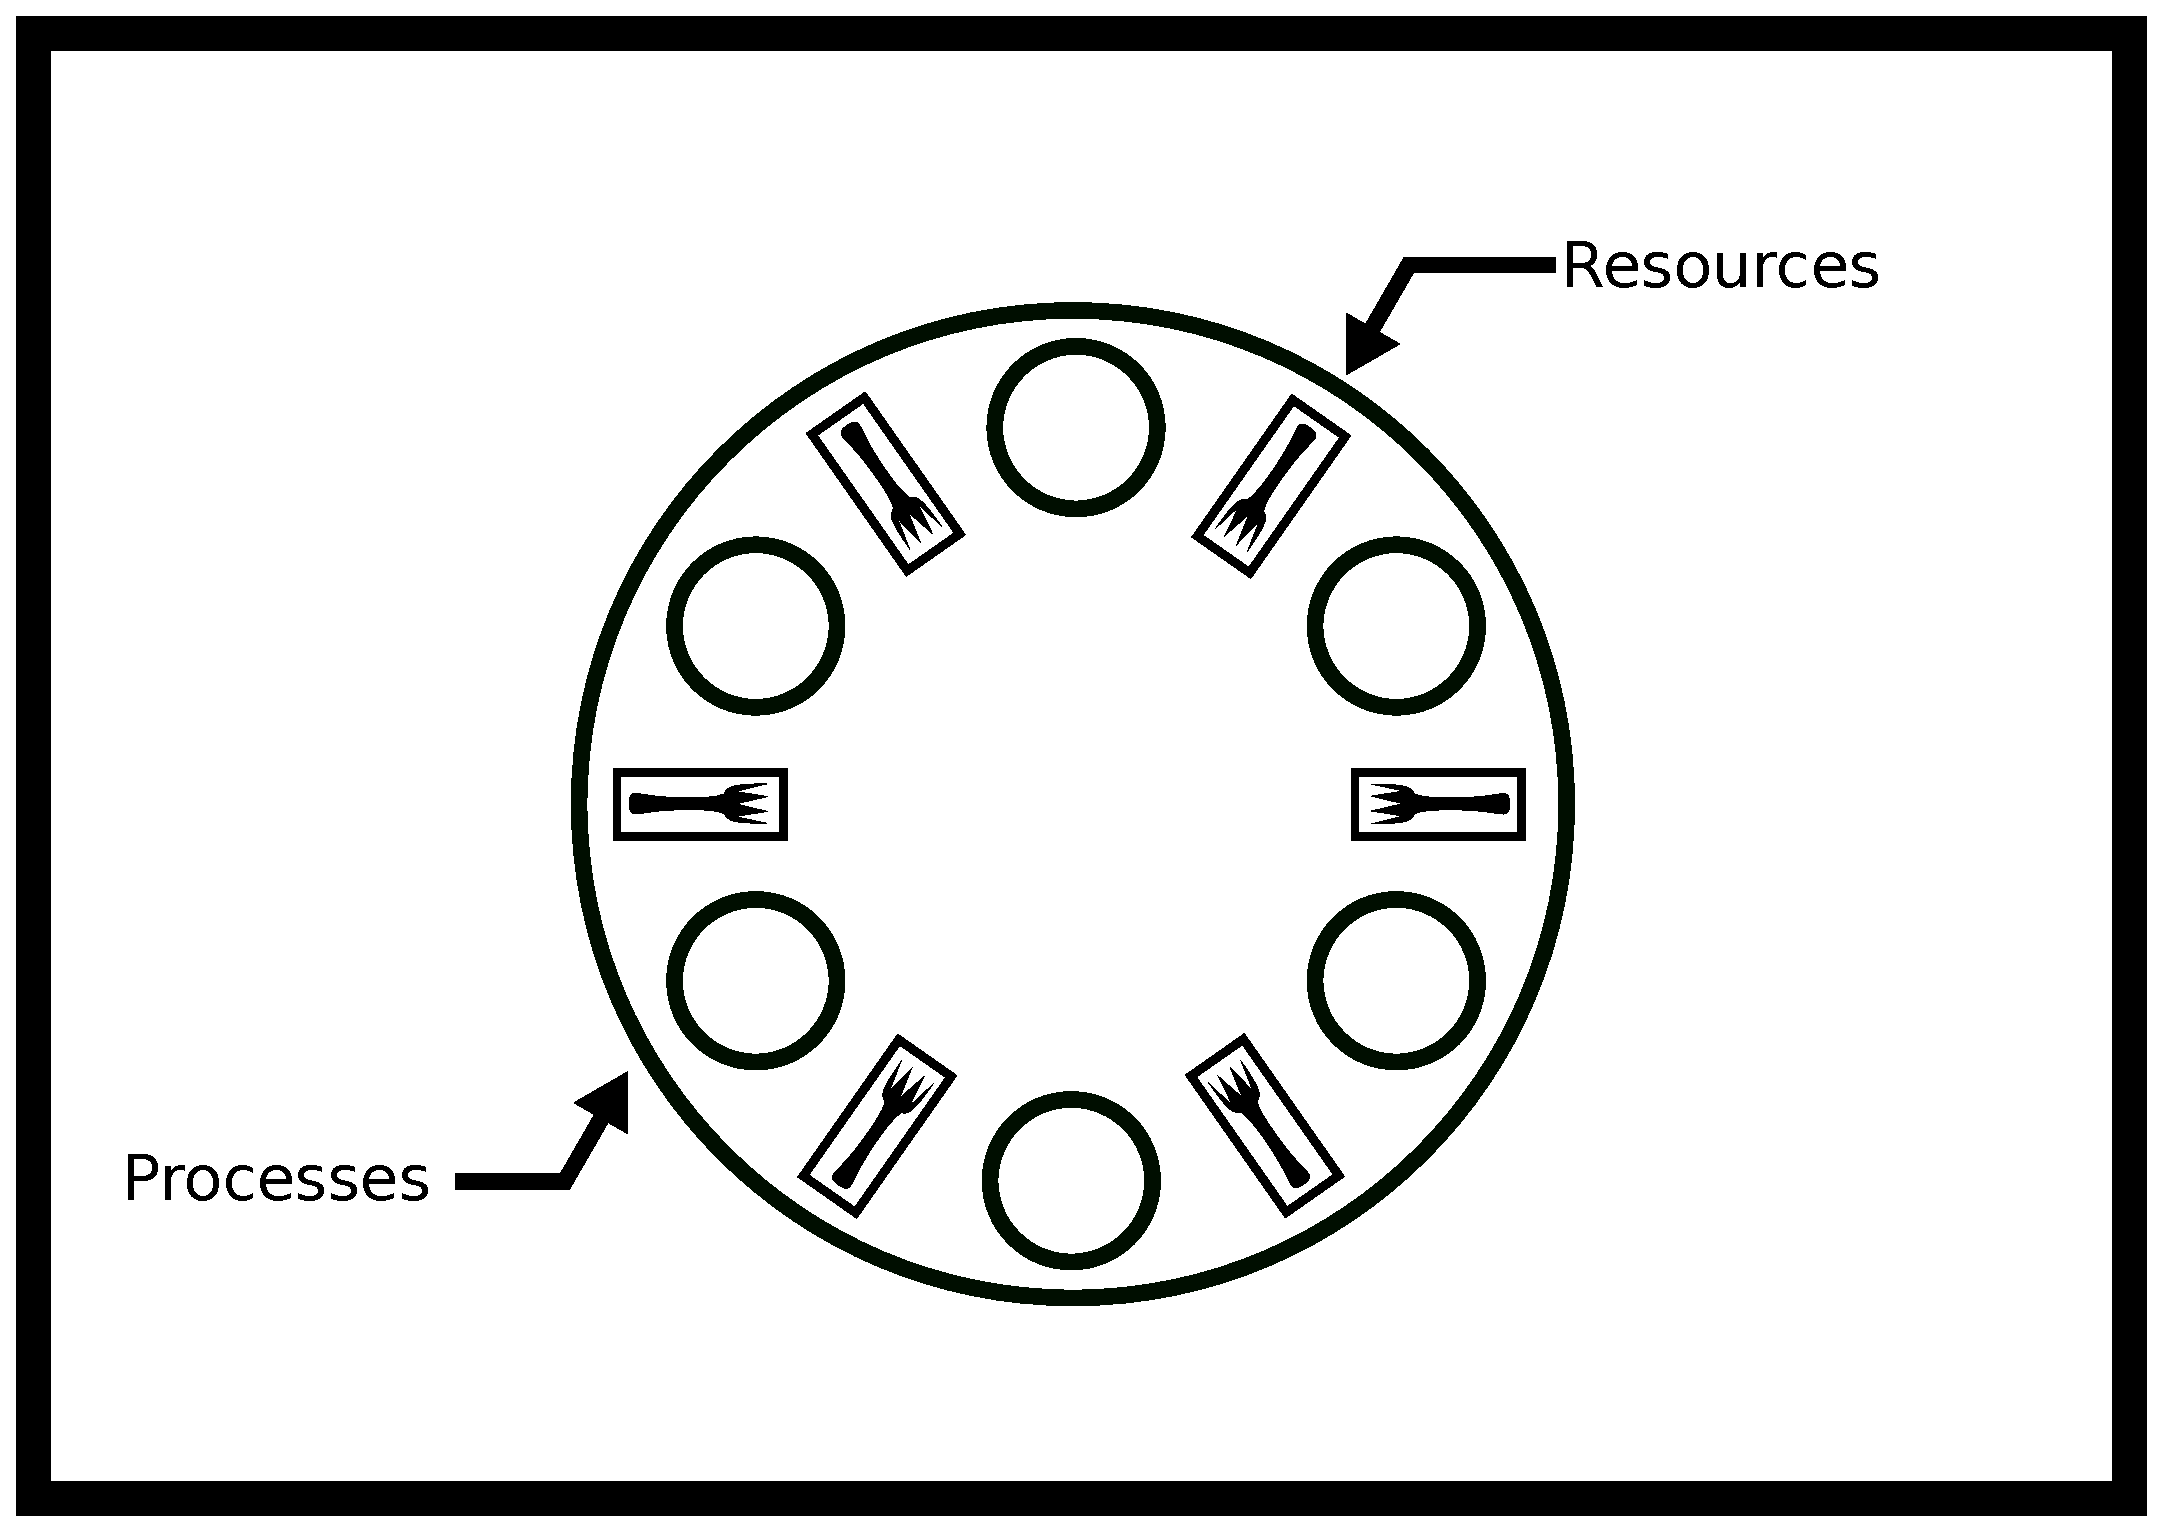
\includegraphics[width=.5\textwidth]{deadlock/drawings/dining.eps}
	\caption{Dining Philosophers}
\end{figure}

Is it possible to design an efficient solution such that all philosophers get to eat?
Or, will some philosophers starve, never obtaining a second chopstick?
Or will all of them deadlock?
For example, imagine each guest picks up the chopstick on their left and then waits for the chopstick on their right to be free.
Oops - our philosophers have deadlocked!
Each philosopher is essentially the same, meaning that each philosopher has the same instruction set based on the other philosopher i.e. you can't tell every even philosopher to do one thing and every odd philosopher to do another thing.

\subsection{Failed Solutions}

\begin{lstlisting}[language=C]
void* philosopher(void* forks){
  info phil_info = forks;
  pthread_mutex_t* left_fork = phil_info->left_fork;
  pthread_mutex_t* right_fork = phil_info->right_fork;
  while(phil_info->simulation){
    pthread_mutex_lock(left_fork);
    pthread_mutex_lock(right_fork);
    eat(left_fork, right_fork);
    pthread_mutex_unlock(left_fork);
    pthread_mutex_unlock(right_fork);
  }
}
\end{lstlisting}

This looks good but.
What if everyone picks up their left fork and is waiting on their right fork? We have deadlocked the program.
It is important to note that deadlock doesn't happen all the time and the probability that this solution deadlock goes down as the number of philosophers goes up.
What is important to note is that eventually that this solution will deadlock, letting threads starve which is bad.
Here is a simple resource allocation graph that shows how the system could be deadlocked

\begin{figure}[H]
	\centering
	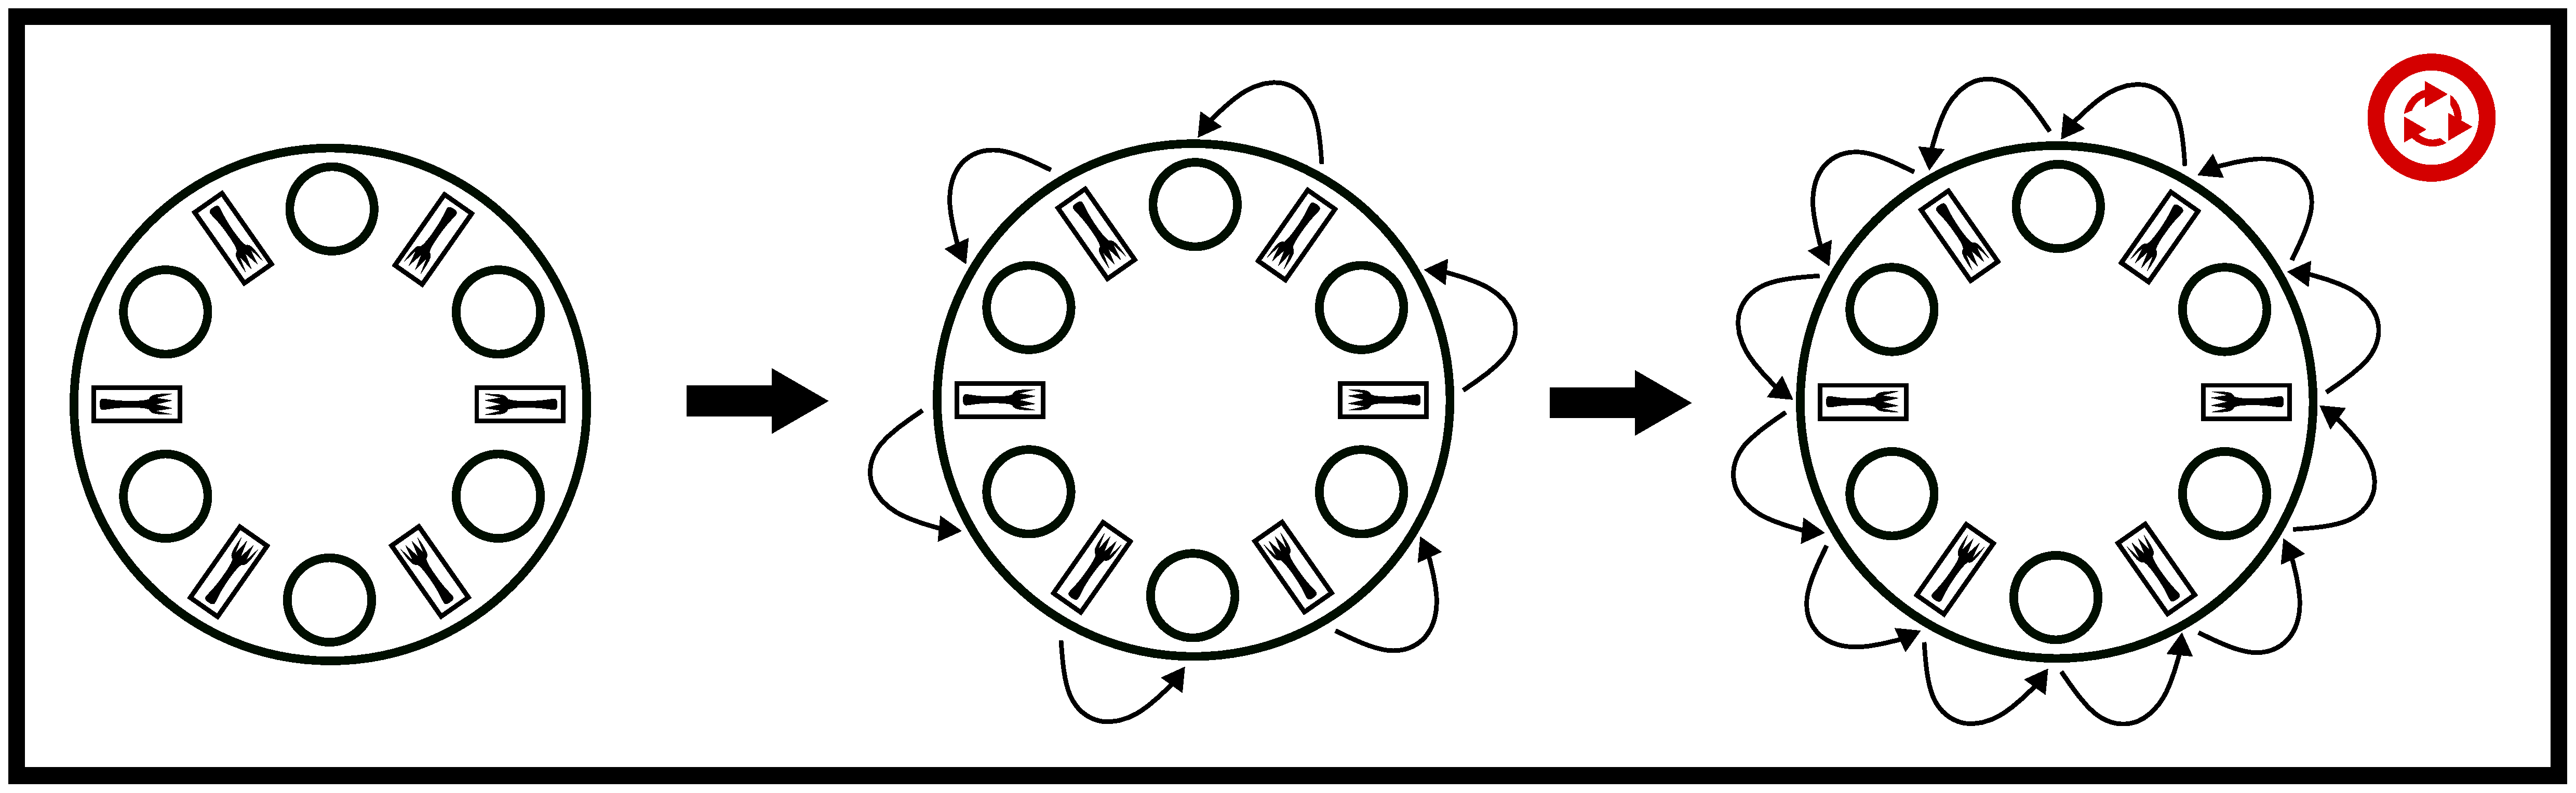
\includegraphics[width=.9\textwidth]{deadlock/drawings/dining_naive.eps}
	\caption{Left right dining philosopher cycle}
\end{figure}


So now you are thinking about breaking one of the Coffman Conditions.
Let's break Hold and Wait!

\begin{lstlisting}[language=C]
void* philosopher(void* forks){
  info phil_info = forks;
  pthread_mutex_t* left_fork = phil_info->left_fork;
  pthread_mutex_t* right_fork = phil_info->right_fork;
  while(phil_info->simulation){
    int left_succeed = pthread_mutex_trylock(left_fork);
    if (!left_succeed) {
      sleep();
      continue;
    }
    int right_succeed = pthread_mutex_trylock(right_fork);
    if (!right_succeed) {
      pthread_mutex_unlock(left_fork);
      sleep();
      continue;
    }
    eat(left_fork, right_fork);
    pthread_mutex_unlock(left_fork);
    pthread_mutex_unlock(right_fork);
  }
}
\end{lstlisting}

Now our philosopher picks up the left fork and tries to grab the right.
If it's available, they eat.
If it's not available, they put the left fork down and try again.
No deadlock! But, there is a problem.
What if all the philosophers pick up their left at the same time, try to grab their right, put their left down, pick up their left, try to grab their right and so on.
Here is what a time evolution of the system would look like.

\begin{figure}[H]
	\centering
	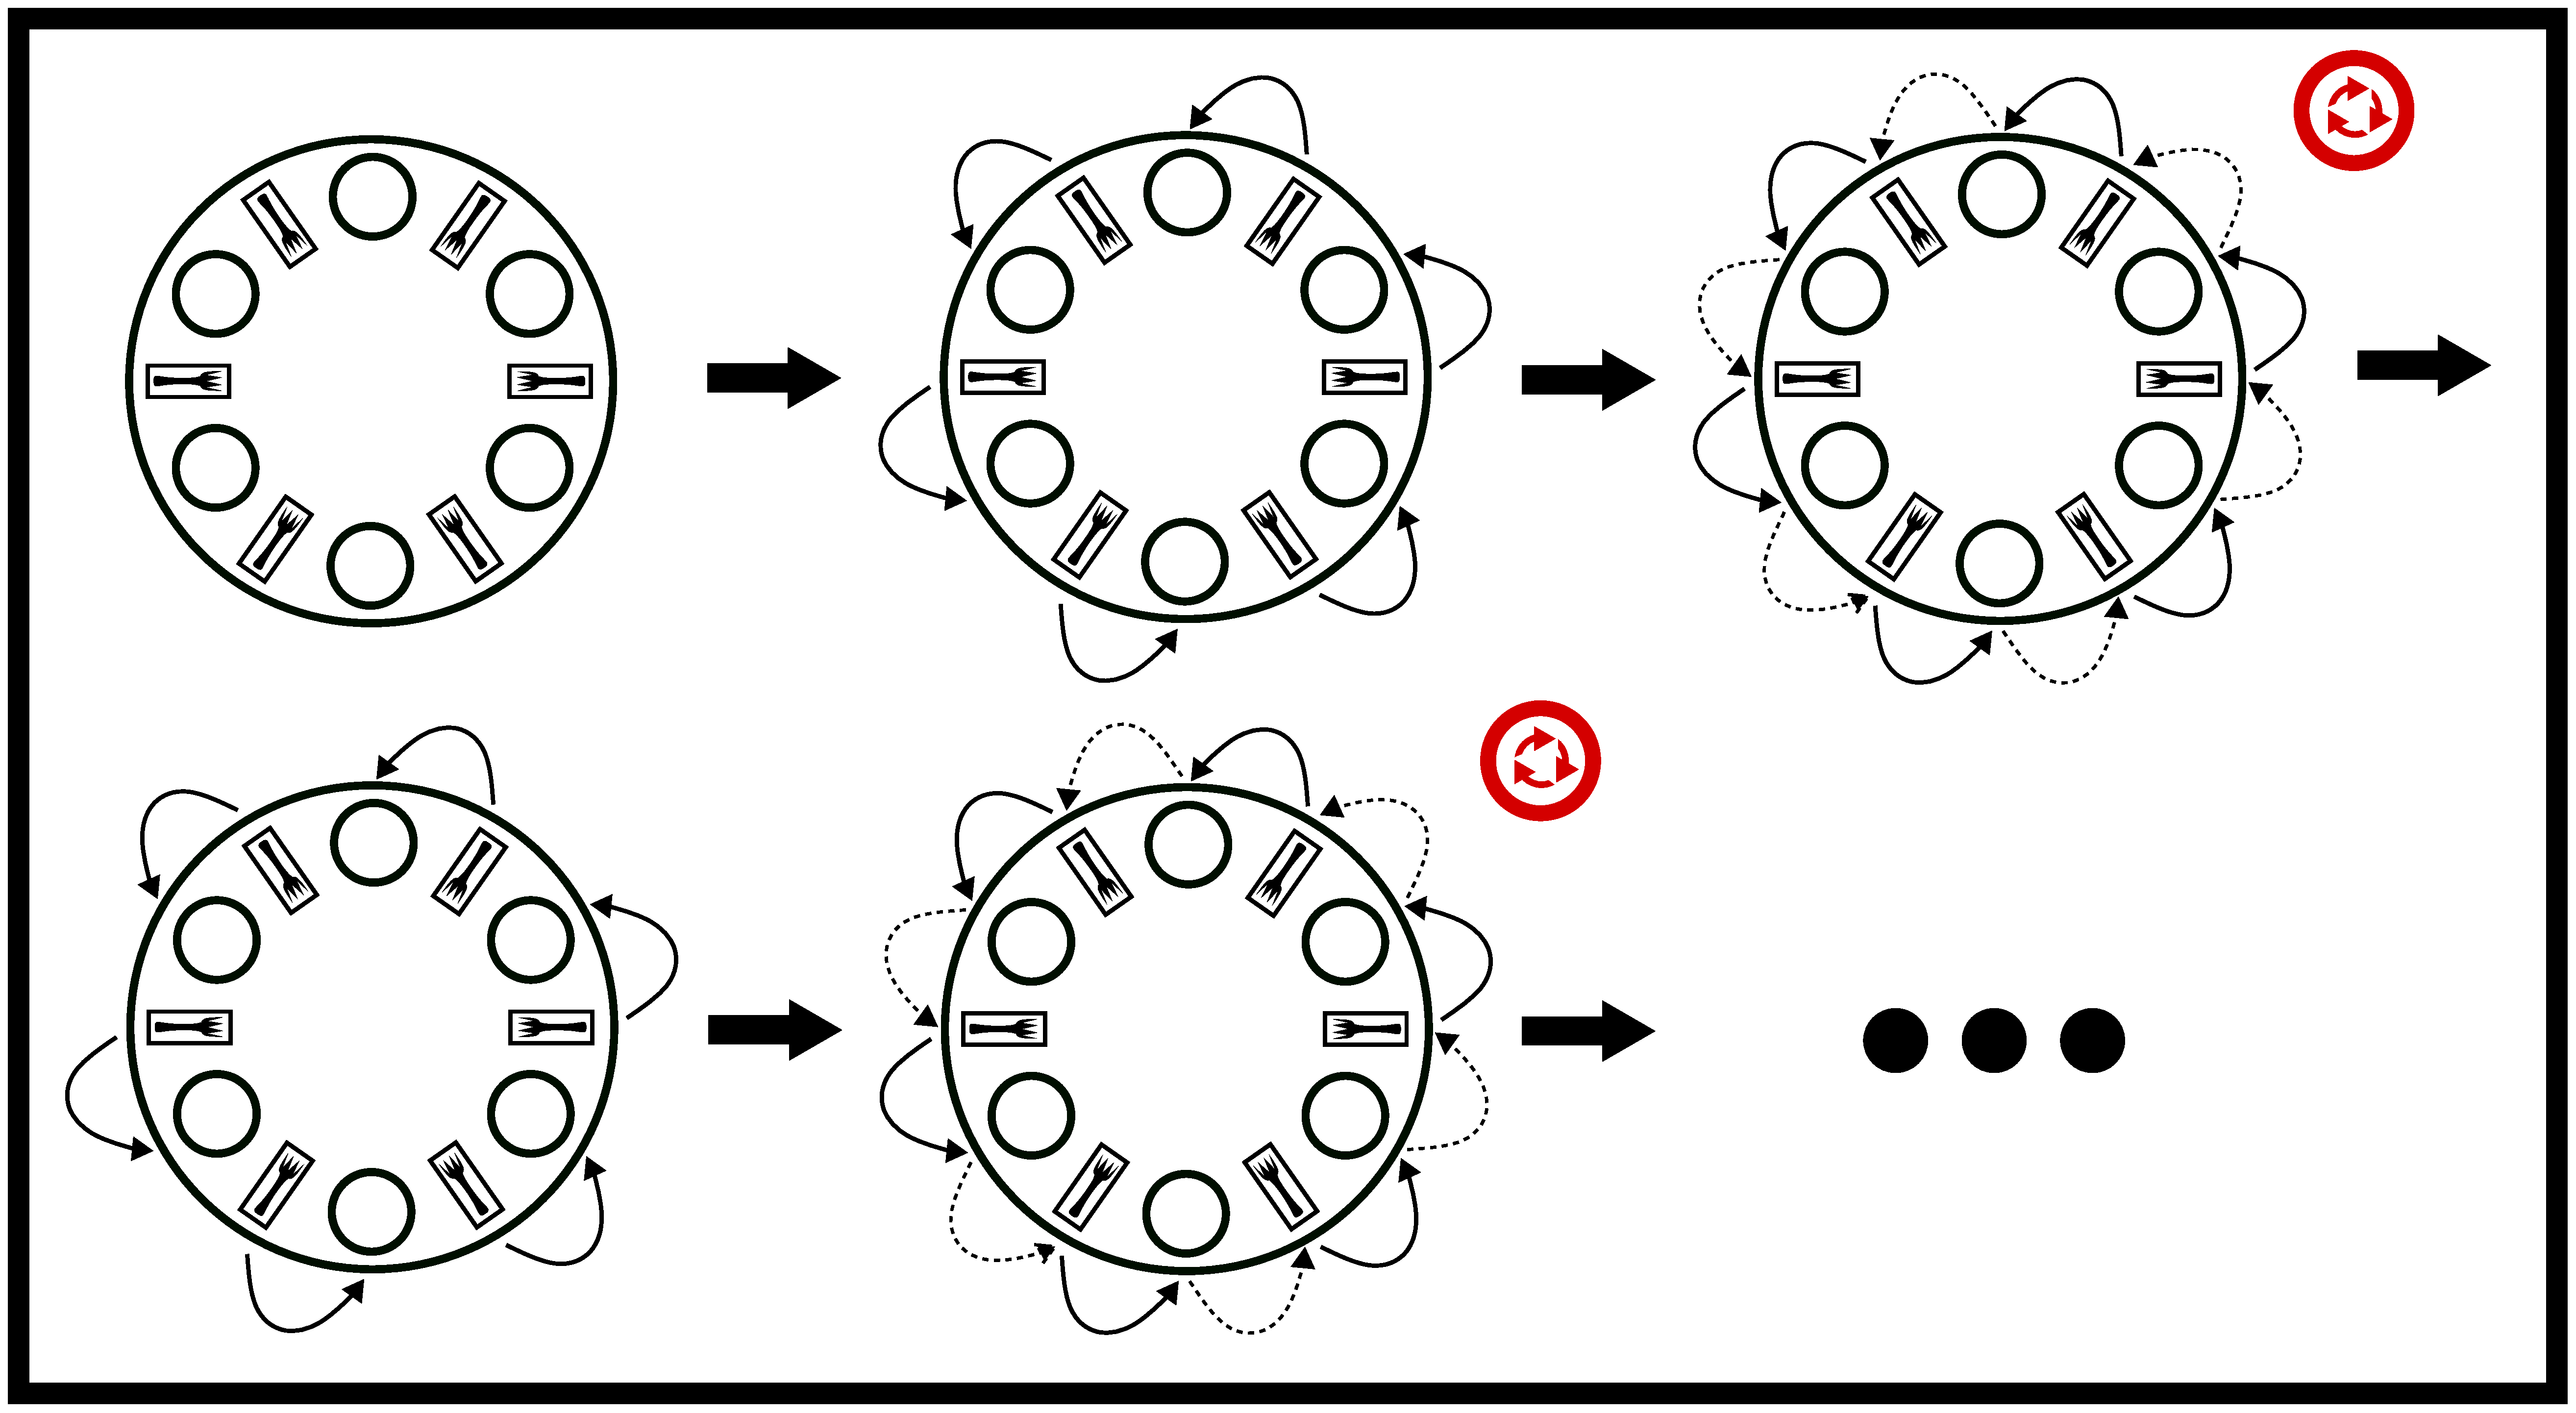
\includegraphics[width=.9\textwidth]{deadlock/drawings/dining_livelock.eps}
	\caption{Livelock Failure}
\end{figure}

We have now livelocked our solution! Our poor philosophers are still starving, so let's give them some proper solutions.

\section{Viable Solutions}

The naive arbitrator solution has one arbitrator a mutex for example.
Have each of the philosophers ask the arbitrator for permission to eat or trylock an arbitrator mutex.
This solution allows one philosopher to eat at a time.
When they are done, another philosopher can ask for permission to eat.
This prevents deadlock because there is no circular wait! No philosopher has to wait for any other philosopher.
The advanced arbitrator solution is to implement a class that determines if the philosopher's forks are in the arbitrator's possession.
If they are, they give them to the philosopher, let him eat, and take the forks back.
This has the bonus of being able to have multiple philosophers eat at the same time.

There are a lot of problems with these solutions.
One is that they are slow and have a single point of failure.
Assuming that all the philosophers are good-willed, the arbitrator needs to be fair.
In practical systems, the arbitrator tends to give forks to the same processes because of scheduling or pseudo-randomness.
Another important thing to note is that this prevents deadlock for the entire system.
But in our model of dining philosophers, the philosopher has to release the lock themselves.
Then, you can consider the case of the malicious philosopher (let's say Descartes because of his Evil Demons) could hold on to the arbitrator forever.
He would make forward progress and the system would make forward progress but there is no way of ensuring that each process makes forward progress without assuming something about the processes or having true preemption -- meaning that a higher authority (let's say Steve Jobs) tells them to stop eating forcibly.


\begin{proof} The arbitrator solution doesn't deadlock
	
	The proof is about as simple as it gets. Only one philosopher can request resources at a time. There is no way to make a cycle in the resource allocation graph with only one philosopher acting in pickup the left then the right fork which is what we needed to show.
	
\end{proof}

\begin{figure}[H]
	\centering
	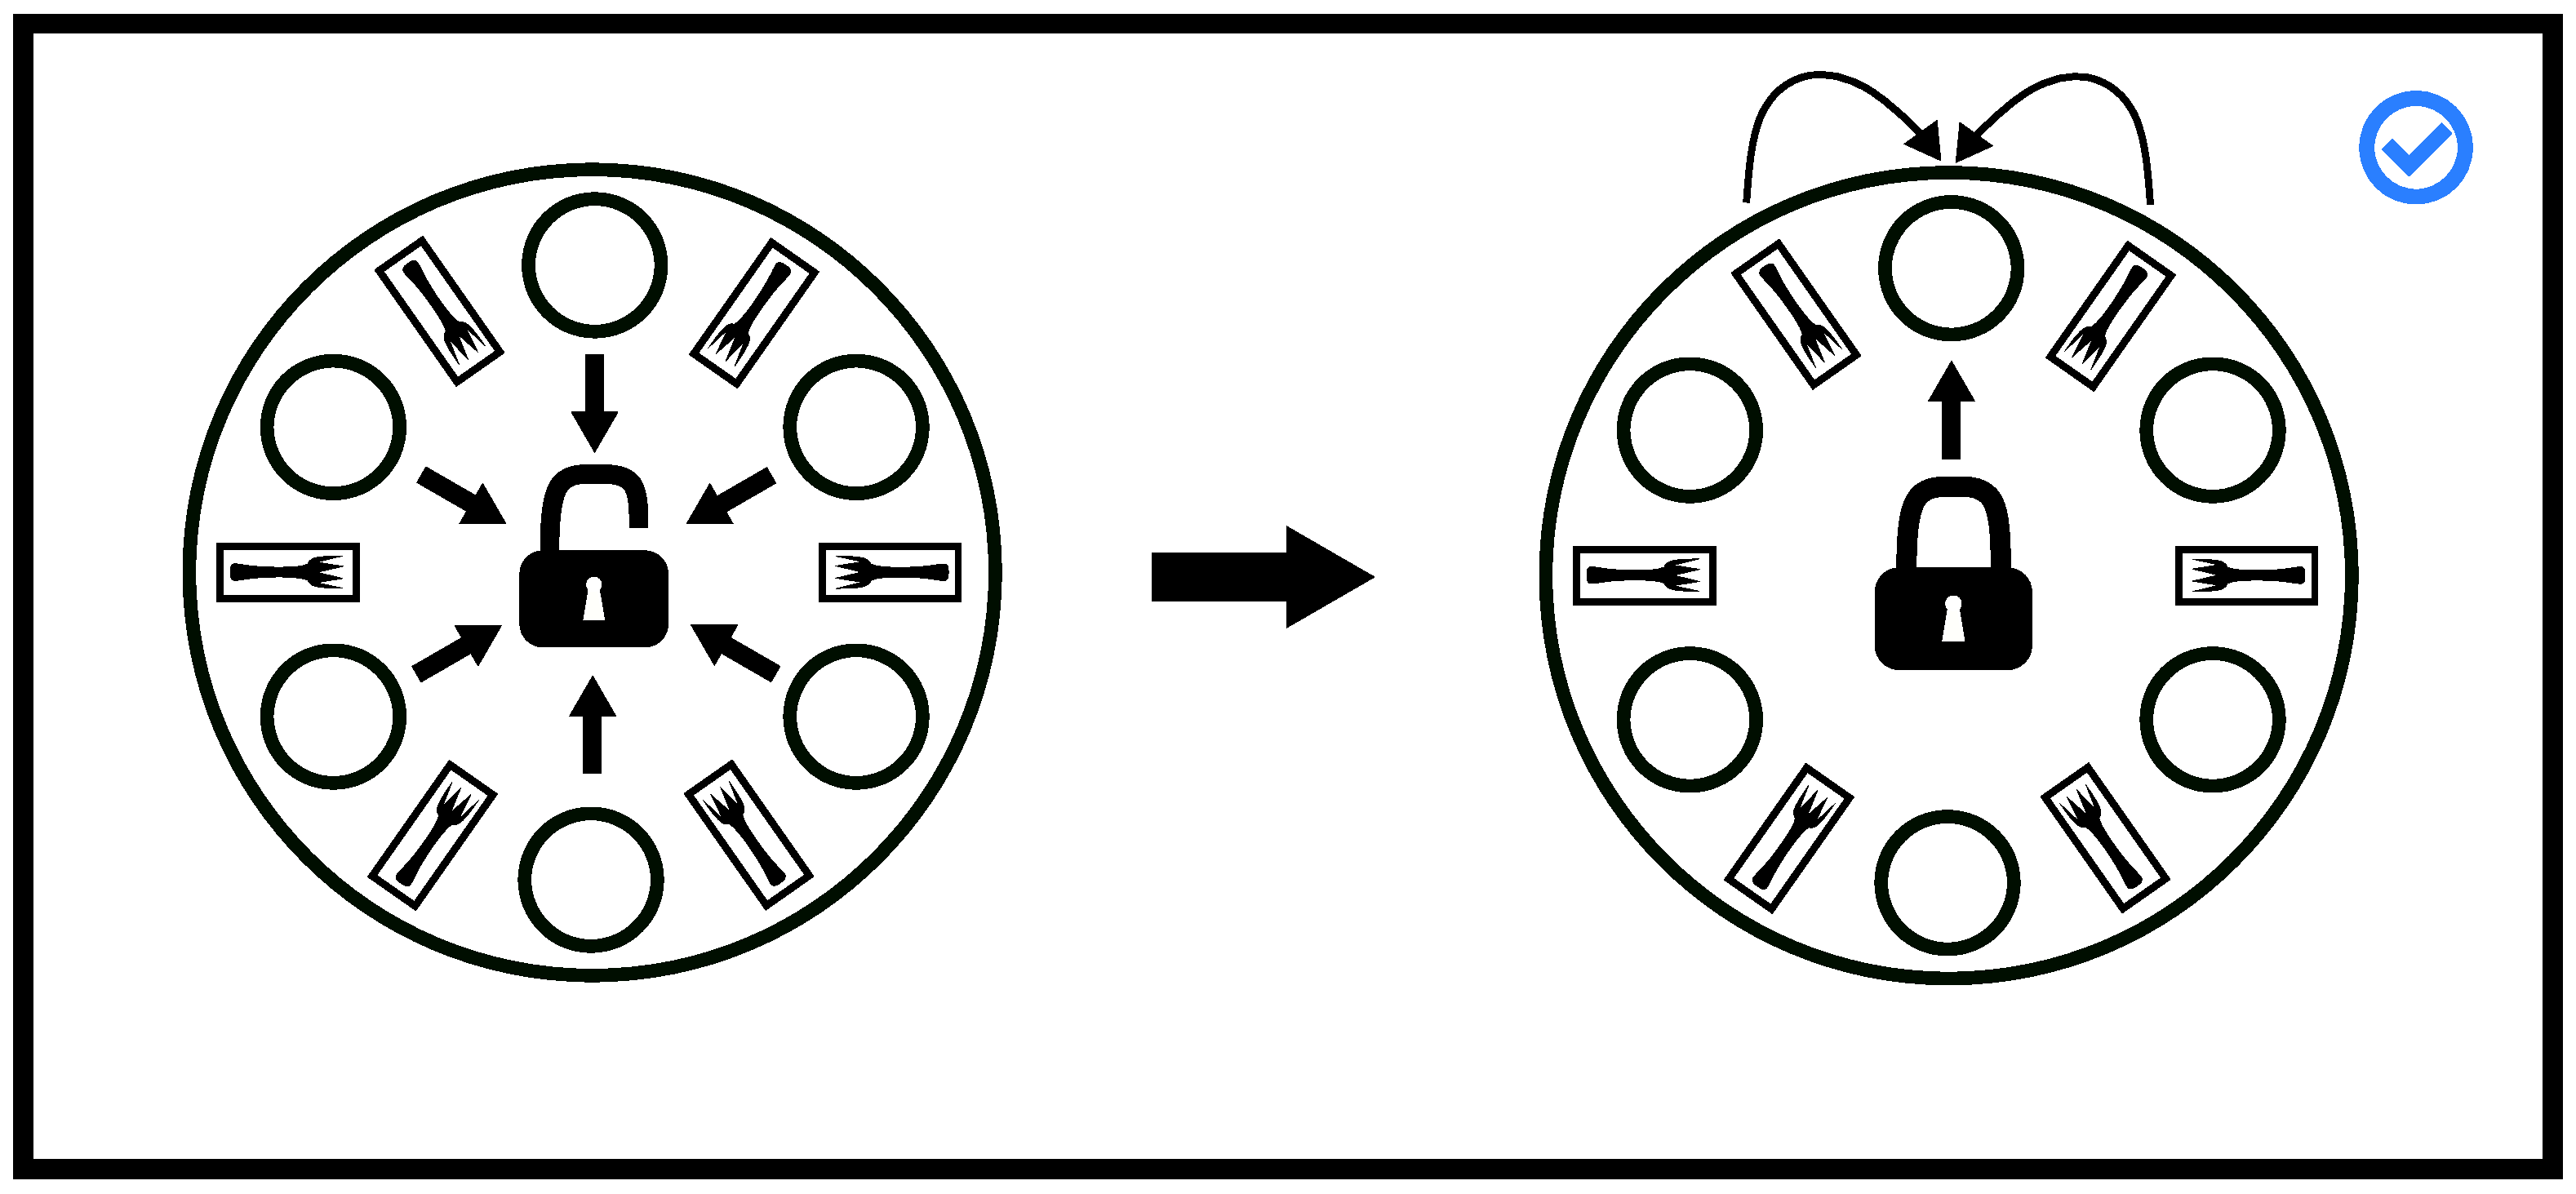
\includegraphics[width=.9\textwidth]{deadlock/drawings/dining_arbitrator.eps}
	\caption{Arbitrator Diagram}
\end{figure}

\subsection{Leaving the Table (Stallings' Solution)}

Why does the first solution deadlock?
Well, there are $n$ philosophers and $n$ chopsticks.
What if there is only 1 philosopher at the table?
Can we deadlock?
No.
How about 2 philosophers?
3?
You can see where this is going.
Stallings' \cite[P. 280]{stalling} solution removes philosophers from the table until deadlock is not possible -- think about what the magic number of philosophers at the table.
The way to do this in the actual system is through semaphores and letting a certain number of philosophers through.
This has the benefit that multiple philosophers can be eating.

In the case that the philosophers aren't evil, this solution requires a lot of time-consuming context switching.
There is also no reliable way to know the number of resources beforehand.
In the dining philosophers case, this is solved because everything is known but trying to specify an operating system where a system doesn't know which file is going to get opened by what process can lead to a faulty solution.
And again since semaphores are system constructs, they obey system timing clocks which means that the same processes tend to get added back into the queue again.
Now if a philosopher becomes evil, then the problem becomes that there is no preemption.
A philosopher can eat for as long as they want and the system will continue to function but that means the fairness of this solution can be low in the worst case.
This works best with timeouts or forced context switches to ensure bounded wait times.

\begin{proof} Stallings' Solution Doesn't Deadlock.
	Let's number the philosophers $\{p_0, p_1, .., p_{n-1}\}$ and the resources $\{r_0, r_1, .., r_{n-1}\}$.
	A philosopher $p_i$ needs resource $r_{i-1 \mod n}$ and $r_{i + 1 \mod n}$.
	Without loss of generality, let us take $p_i$ out of the picture.
	Each resource had exactly two philosophers that could use it.
	Now resources $r_{i-1 \mod n}$ and $r_{i + 1 \mod n}$ only have on philosopher waiting on it.
	Even if hold and wait, no preemption, and mutual exclusion or present, the resources can never enter a state where one philosopher requests them and they are held by another philosopher because only one philosopher can request them.
	Since there is no way to generate a cycle otherwise, circular wait cannot hold.
	Since circular wait cannot hold, deadlock cannot happen.
\end{proof}

Here is a visualization of the worst-case.
The system is about to deadlock, but the approach resolves it.

\begin{figure}[H]
	\centering
	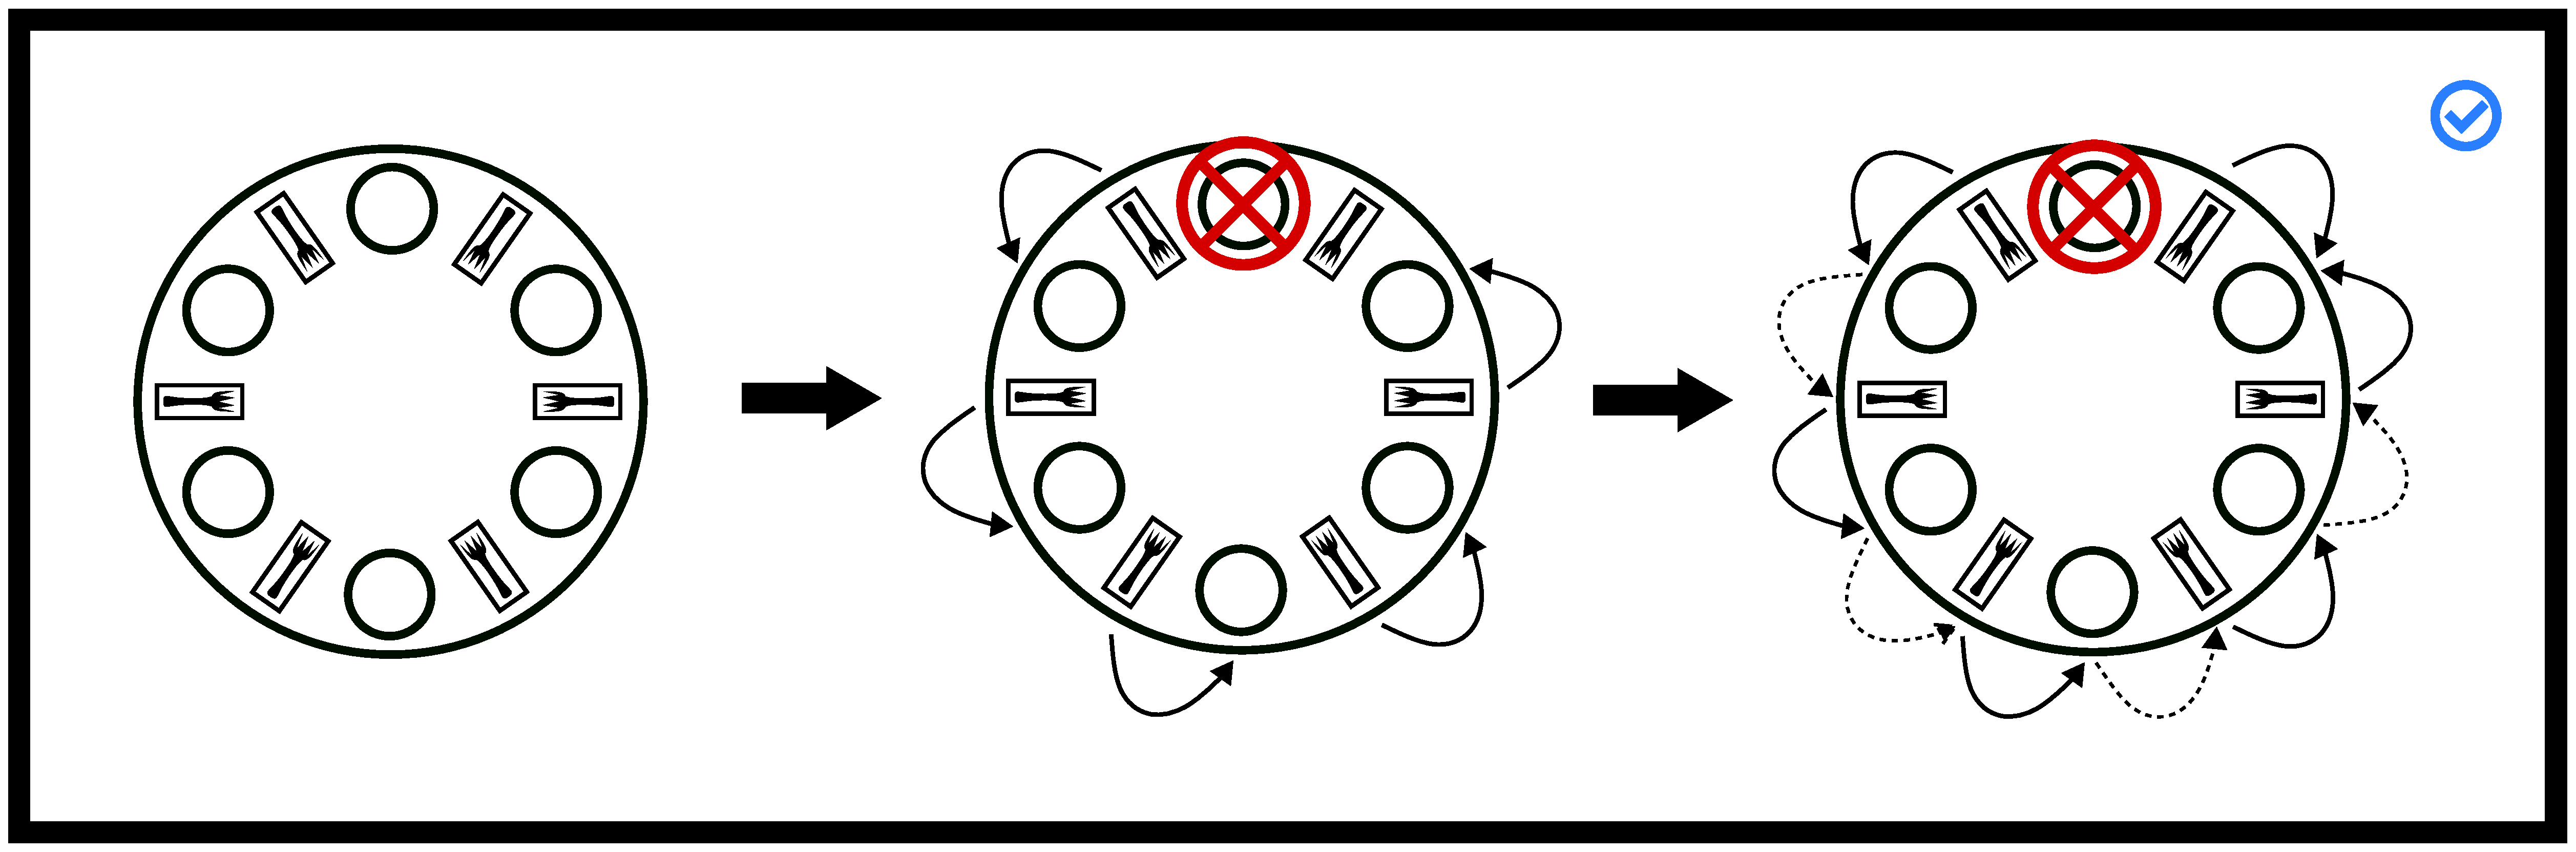
\includegraphics[width=.9\textwidth]{deadlock/drawings/dining_stalling.eps}
	\caption{Stalling solution almost deadlock}
\end{figure}


\subsection{Partial Ordering (Dijkstra's Solution)}

This is Dijkstra's solution \cite[P. 20]{EWD:EWD310}. He was the one to propose this problem on an exam.
Why does the first solution deadlock? Dijkstra thought that the last philosopher who picks up his left fork (causing the solution to deadlock) should pick up his right.
He accomplishes it by number the forks $1..n$, and tells each of the philosophers to pick up his lower number fork.
Let's run through the deadlock condition again.
Everyone tries to pick up their lower number fork first.
Philosopher $1$ gets fork $1$, Philosopher $2$ gets fork $2$, and so on until we get to Philosopher $n$.
They have to choose between fork $1$ and $n$.
fork $1$ is already held up by philosopher $1$, so they can't pick up that fork, meaning he won't pick up fork $n$.
We have broken \keyword{circular wait}! Meaning deadlock isn't possible.

Some problems are that an entity either needs to know the finite set of resources in advance or be able to produce a consistent partial order suck that circular wait cannot happen.
This also implies that there needs to be some entity, either the operating system or another process, deciding on the number and all of the philosophers need to agree on the number as new resources come in.
As we have also seen with previous solutions, this relies on context switching.
This prioritizes philosophers that have already eaten but can be made fairer by introducing random sleeps and waits.

\begin{proof} Dijkstra's Solution Doesn't Deadlock
	
	The proof is similar to the previous proof.
	Let's number the philosophers $\{p_0, p_1, .., p_{n-1}\}$ and the resources $\{r_0, r_1, .., r_{n-1}\}$.
	A philosopher $p_i$ needs resource $r_{i-1 \mod n}$ and $r_{i + 1 \mod n}$.
	Each philosopher will grab $r_{i-1 \mod n}$ then $r_{i + 1 \mod n}$ but the last philosopher will grab in the reverse order.
	Even if hold and wait, no preemption, and mutual exclusion or present.
	Since the last philosopher will grab $r_{n-1}$ then $r_0$ there are two cases either the philosopher has the first lock or the philosopher doesn't.
	
	If the last philosopher $p_{n-1}$ holds the first lock meaning the previous philosopher $p_{n-2}$ is waiting on $r_{n-1}$ meaning $r_{n-2}$ is available.
	Since no other blockers, the philosopher previous $p_{n-3}$ will grab her first lock.
	This is now a reduction to the previous proof of stalling because we now have $n$ resources but only $n-1$ philosophers, meaning this cannot deadlock.
	
	If the philosopher doesn't obtain that first lock, then we have a reduction to Stalling's proof above because now have $n-1$ philosophers vying for $n$ resources.
	Since we can't reach deadlock in either case, this solution cannot deadlock which is what we needed to show.
	
\end{proof}

\begin{figure}[H]
	\centering
	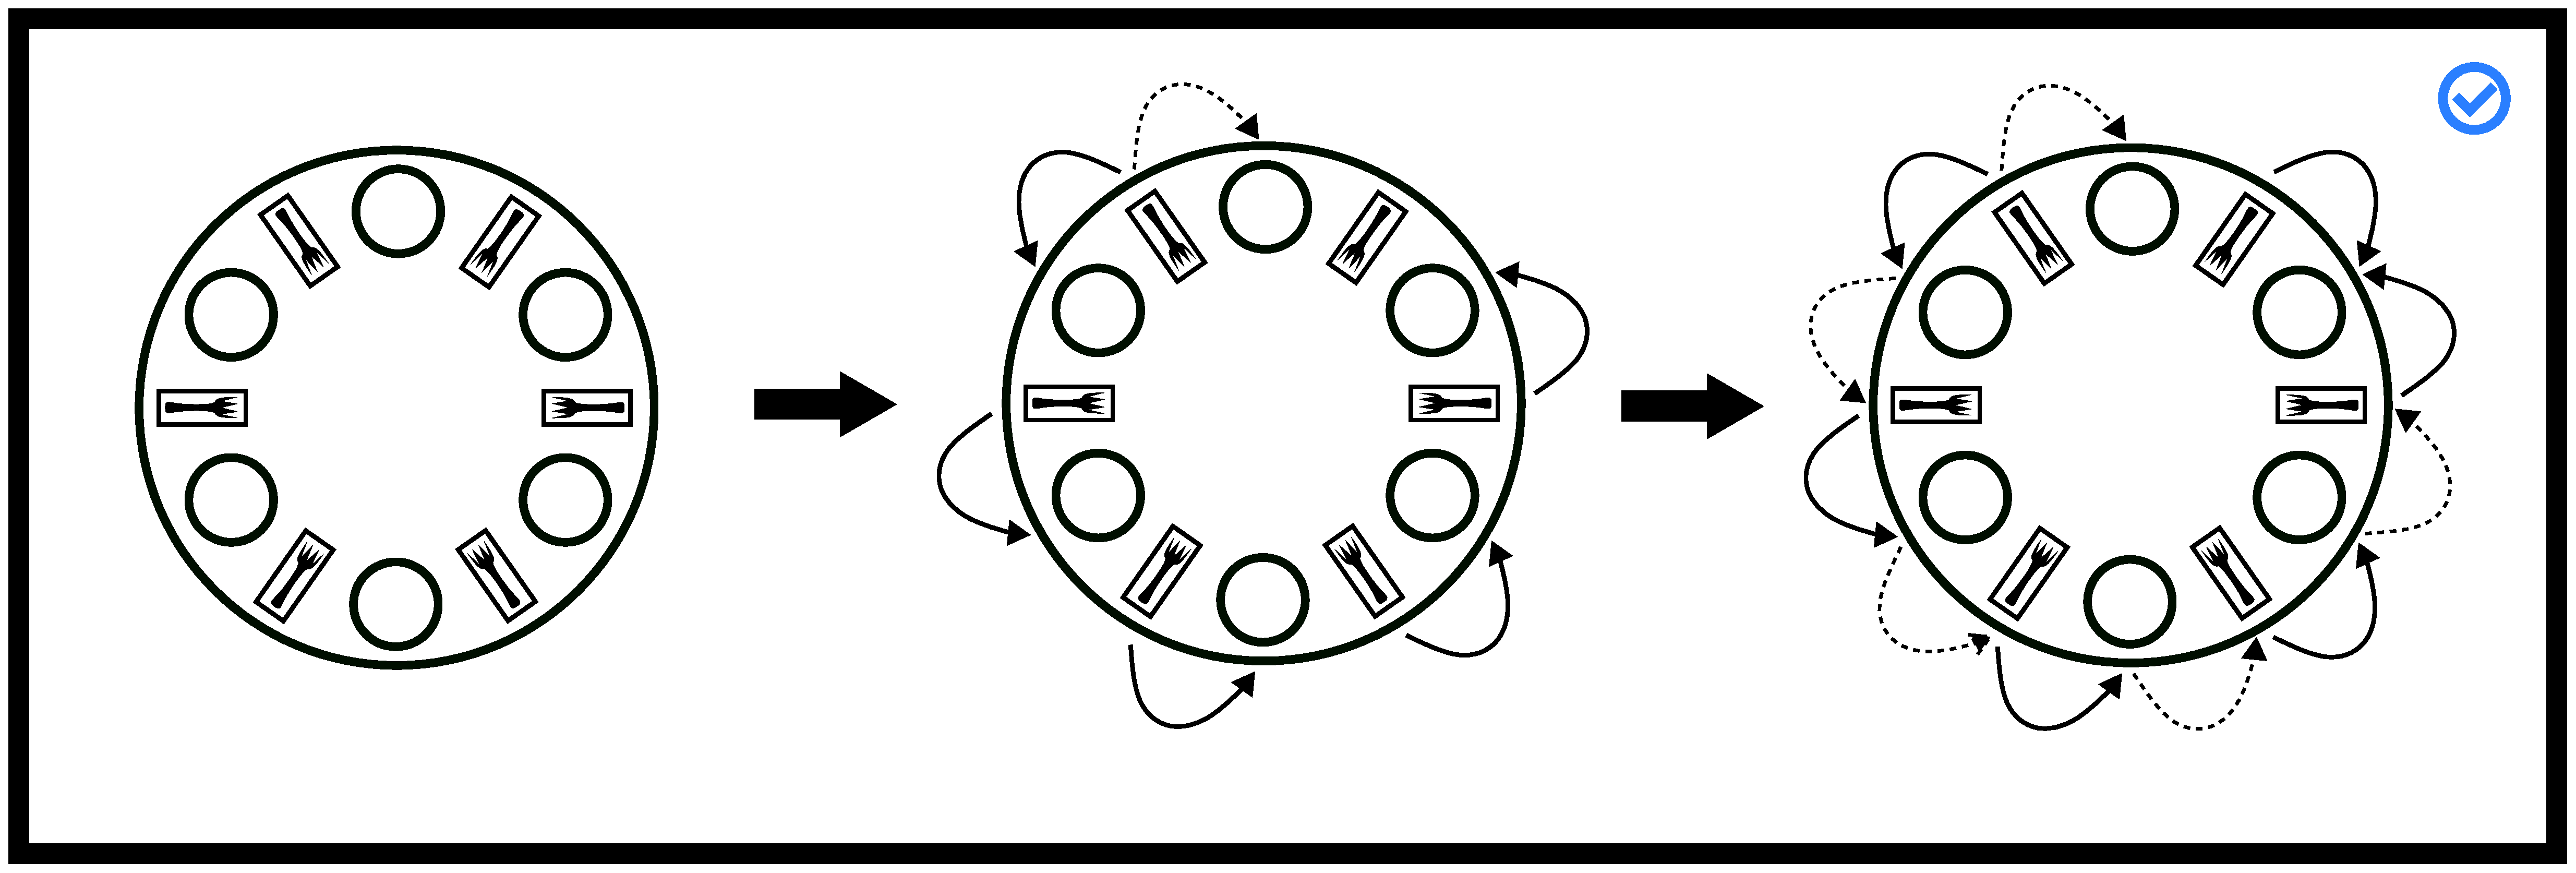
\includegraphics[width=.9\textwidth]{deadlock/drawings/dining_partial.eps}
	\caption{Stalling solution partial deadlock}
\end{figure}

\subsection{Extra: Clean/Dirty Forks (Chandy/Misra Solution)}

There are many more advanced solutions.
One such solution is by Chandy and Misra \cite{Chandy:1984:DPP:1780.1804}.
This is not a true solution to the dining philosophers problem because it has the requirement that philosophers can speak to each other.
It is a solution that ensures fairness for some notion of fairness.
In essence, it defines a series of rounds that a philosopher must eat in a given round before going to the next one.

We won't detail the proof here because it is a little more involved, but feel free to read more.

\subsection{Extra: Actor Model}

The actor model is another form of synchronization that doesn't have to do anything with negotiating locks or waiting.
The idea is simple.
Each actor can either perform work, create more actors, send messages, or respond to messages.
Any time an actor needs something from another actor, it sends a message.
Most importantly, an actor is only responsible for one thing.
If we were implementing a real-world application, we may have an actor that handles the database, one that handles the incoming connections, one that services the connections, etc.
These actors would pass messages to each other like ``there is a new connection'' from the incoming connection actor to the servicing actor.
The servicing actor may send a data request message to the database actor and a data response message comes back.

While this seems like the perfect solution there are drawbacks.
The first is the actual library of communication needs to be synchronized.
If you don't have a framework that does this already -- like the Message Passing Interface or MPI for High-Performance Computing -- then the framework will have to be built and would most likely be as much work to build efficiently compared to direct synchronization.
Also, the messages now encounter additional overhead for serializing and deserializing or at the least.
And a final drawback is that an actor could take an arbitrarily long time to respond to a message, spurring the need for shadow actors who service the same job.

As mentioned, there are frameworks like \href{https://en.wikipedia.org/wiki/Message\_Passing\_Interface}{Message passing interface} that is somewhat based on the actor model and allows distributed systems in high-performance computing to work effectively, but your mileage may vary
If you want to read further on the model, feel free to glance over the Wikipedia page listed below.
\href{https://en.wikipedia.org/wiki/Actor\_model}{Further reading on the actor model}

\section{Topics}

\begin{itemize}
	\item Coffman Conditions
	\item Resource Allocation Graphs
	\item Dining Philosophers
	\item Failed DP Solutions
	\item Livelocking DP Solutions
	\item Working DP Solutions: Benefits/Drawbacks
	\item \href{http://adit.io/posts/2013-05-11-The-Dining-Philosophers-Problem-With-Ron-Swanson.html}{Ron Swanson Deadlock}
\end{itemize}

\section{Questions}

\begin{itemize}
	\item
	      What are the Coffman conditions?
	\item
	      What does each of the Coffman conditions mean? Define each one.
	\item
	      Give a real-life example of breaking each Coffman condition in turn. A situation to consider: Painters, Paint, Paint Brushes etc. How would you assure that work would get done?
	\item
	      Which Coffman condition is unsatisfied in the following snippet?
	      
	      \begin{lstlisting}[language=C]
// Get both locks or none
pthread_mutex_lock(a);
if(pthread_mutex_trylock( b )) { /* failure */
  pthread_mutex_unlock( a );
}
	      \end{lstlisting}
	\item
	      The following calls are made
	      
	      \begin{lstlisting}[language=c]
// Thread 1
pthread_mutex_lock(m1) // success
pthread_mutex_lock(m2) // blocks

// Thread 2
pthread_mutex_lock(m2) // success
pthread_mutex_lock(m1) // blocks
	      \end{lstlisting}
	      
	      What happens and why? What happens if a third thread calls
	      \keyword{pthread\_mutex\_lock(m1)} ?
	\item
	      How many processes are blocked? As usual, assume that a process can complete if it can acquire all of the resources listed
	      below.
	      
	      \begin{itemize}
	      	\tightlist
	      	\item
	      	      P1 acquires R1
	      	\item
	      	      P2 acquires R2
	      	\item
	      	      P1 acquires R3
	      	\item
	      	      P2 waits for R3
	      	\item
	      	      P3 acquires R5
	      	\item
	      	      P1 waits for R4
	      	\item
	      	      P3 waits for R1
	      	\item
	      	      P4 waits for R5
	      	\item
	      	      P5 waits for R1
	      \end{itemize}
\end{itemize}

Draw out the resource graph!

\bibliographystyle{plainnat}
\bibliography{deadlock/deadlock}
